\section{Overview}\label{sec:overview}

A fixed, armoured desk stand for a 22'' monitor, designed to live in \textbf{portrait} most of the time and
switch to landscape in a couple of minutes. It is printed in six parts in white PLA+, joined with M5 screws into
brass heat-set inserts, and finished by painting a few recessed lines blue, red and yellow.

\begin{center}
\begin{tabularx}{\linewidth}{@{}XXXX@{}}
\kpicard{6}{printed parts}{All fit a 220\,×\,220\,mm bed. No supports.} &
\kpicard{12}{M5 inserts}{4 base · 4 column · 4 head} &
\kpicard{16}{screws}{12 × M5 + 4 × M4 for the monitor} &
\kpicard{300\,mm}{mount height}{Centre of the VESA plate above the desk} \\
\end{tabularx}
\end{center}

\begin{figure}[H]
  \centering
  \begin{subfigure}{0.49\linewidth}\centering
    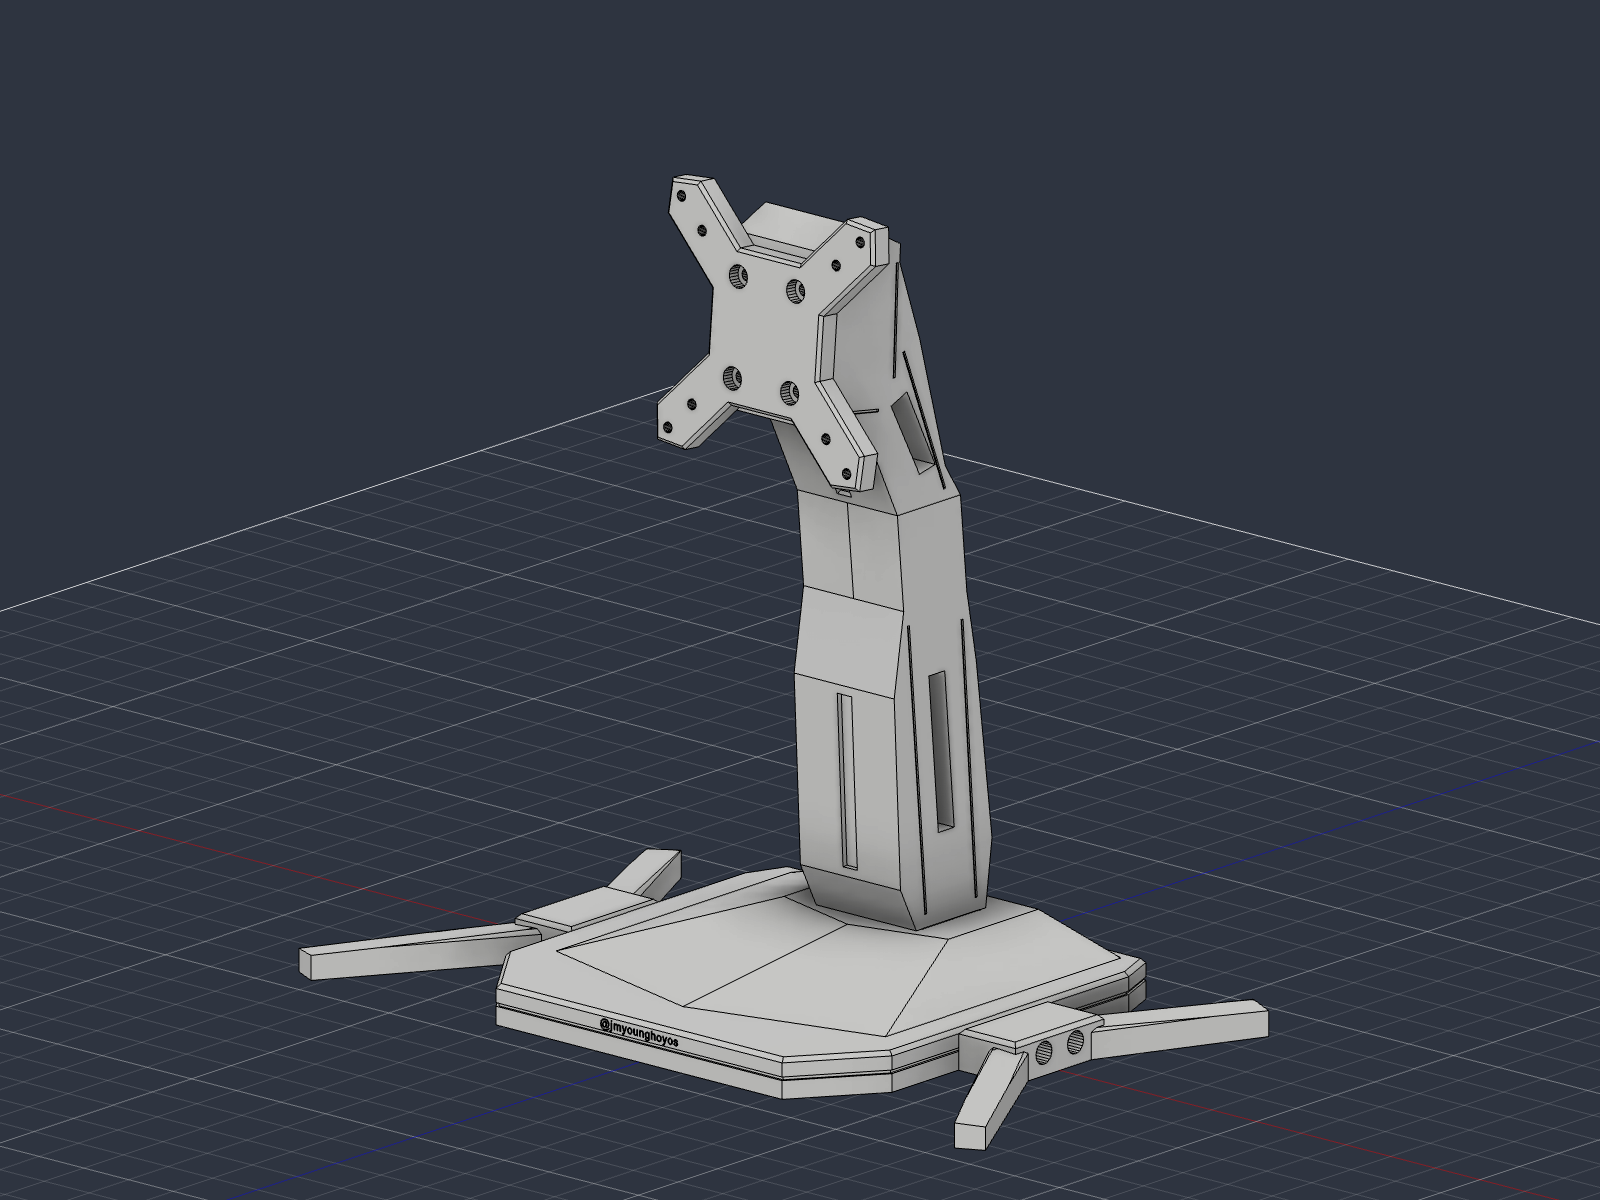
\includegraphics[width = \linewidth]{assembly-front.png}\caption{Front, three-quarter view.}
  \end{subfigure}\hfill
  \begin{subfigure}{0.49\linewidth}\centering
    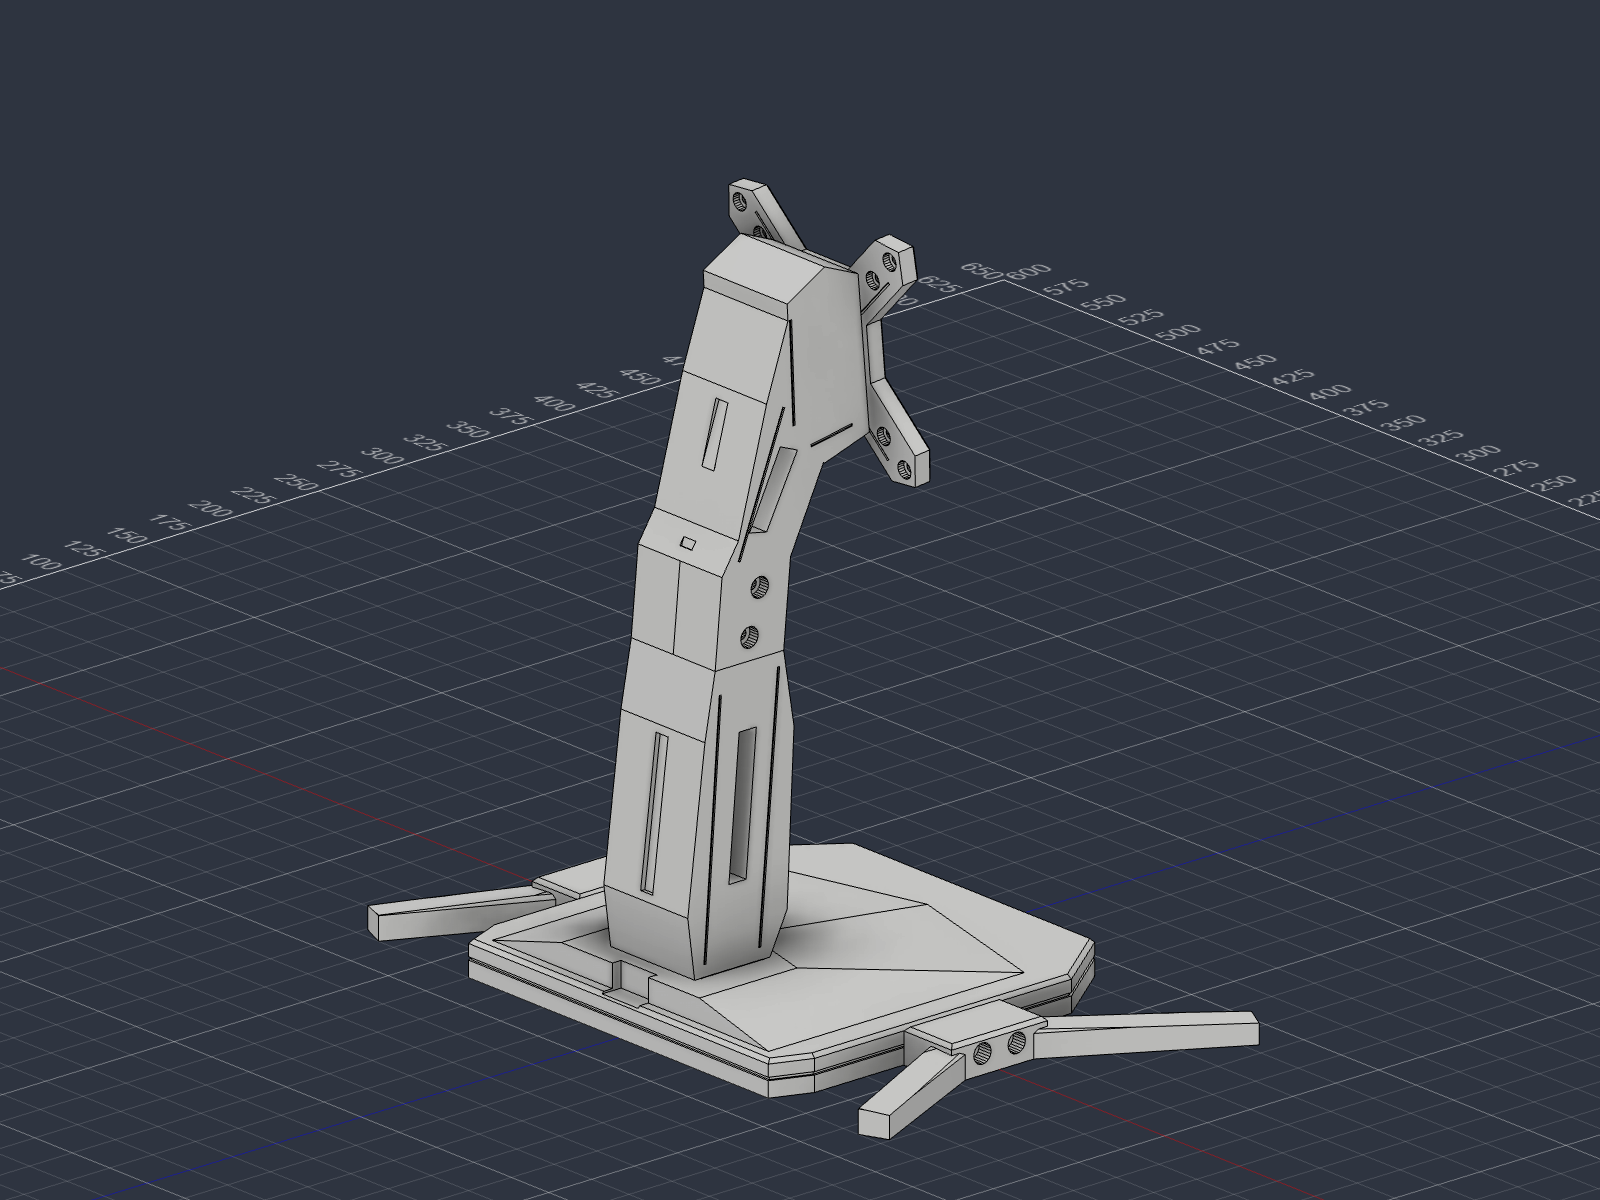
\includegraphics[width = \linewidth]{assembly-back.png}\caption{Back view.}
  \end{subfigure}
  \caption{The assembled stand.}\label{fig:assembly}
\end{figure}

\subsection{Key dimensions}

\begin{table}[H]
\centering
\caption{Main dimensions with the monitor mounted.}
\zebra
\begin{tabularx}{\linewidth}{@{}L{6cm}Y@{}}
\toprule
\thd{Item} & \thd{Value} \\
\midrule
Footprint with feet          & 384\,mm wide × 212\,mm deep (base alone 216 × 208\,mm) \\
Screen tilt                  & 5° backwards (fixed) \\
VESA plate centre            & 300\,mm above the desk \\
Portrait (screen 294 × 488\,mm) & Bottom edge 56\,mm, top edge 544\,mm above the desk \\
Landscape (screen 488 × 294\,mm) & Bottom edge 153\,mm, top edge 447\,mm above the desk \\
Monitor                      & Samsung LS22C310, 488.4 × 294.2 × 41.1\,mm, 2.0\,kg without its stand \\
\bottomrule
\end{tabularx}
\end{table}

\subsection{The six parts}

\begin{figure}[H]
  \centering
  \begin{subfigure}{0.32\linewidth}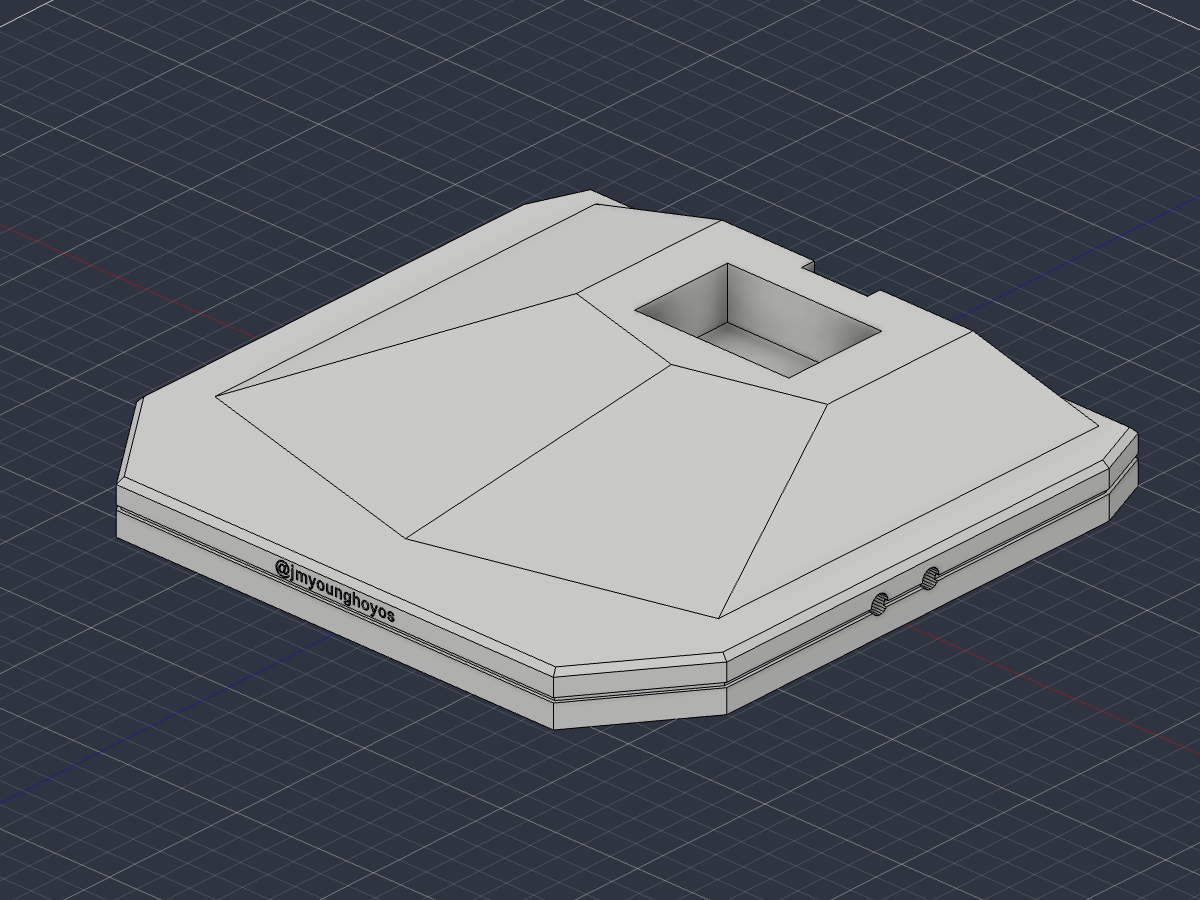
\includegraphics[width = \linewidth]{part-base.png}\caption{01 Base}\end{subfigure}\hfill
  \begin{subfigure}{0.32\linewidth}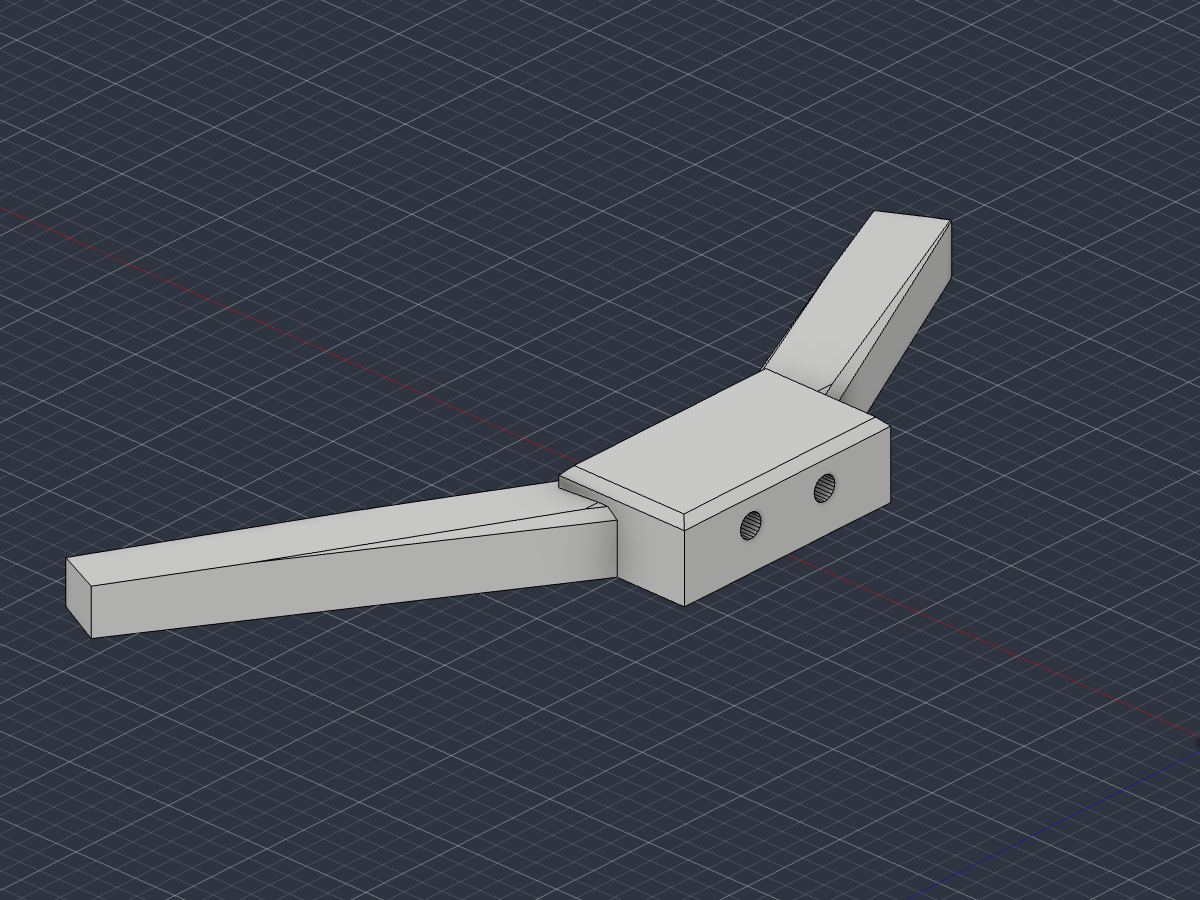
\includegraphics[width = \linewidth]{part-foot-left.png}\caption{02 Foot, left}\end{subfigure}\hfill
  \begin{subfigure}{0.32\linewidth}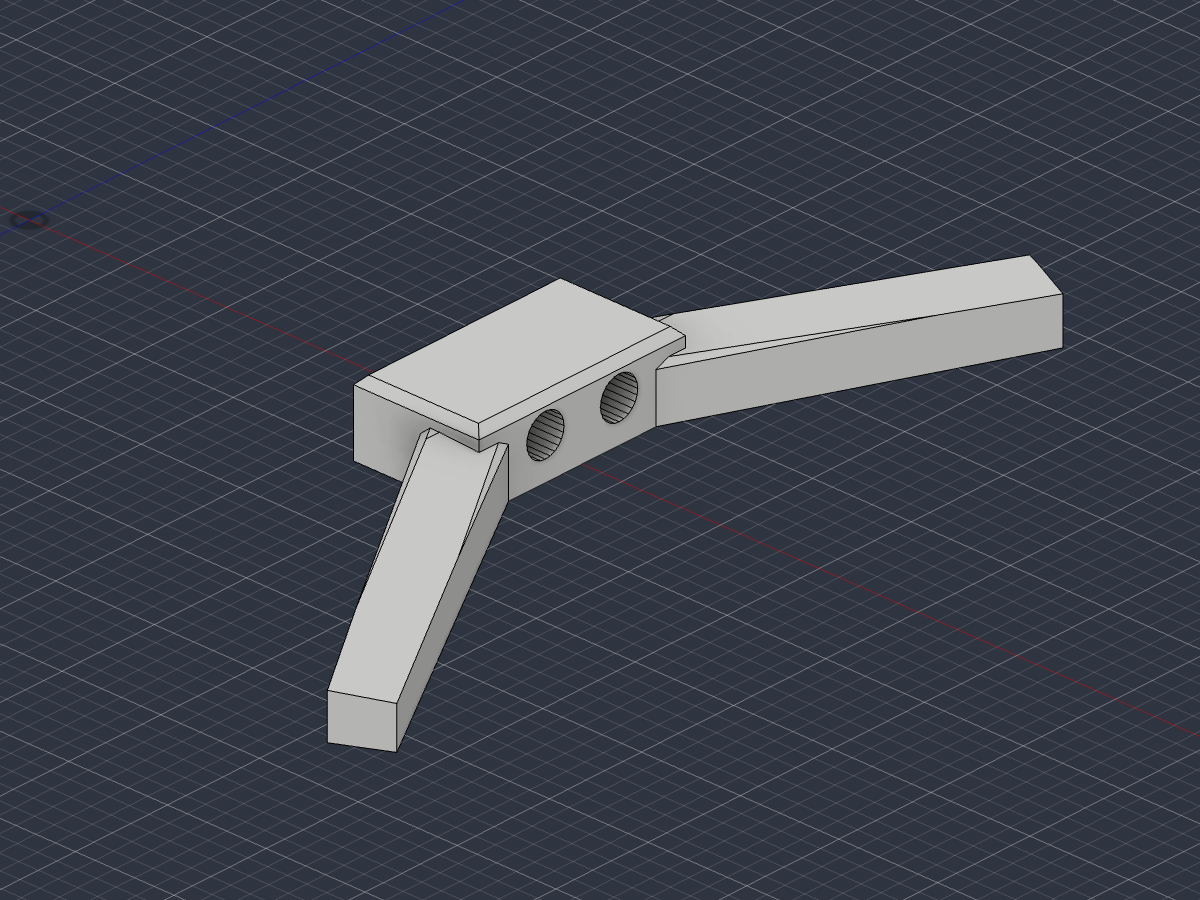
\includegraphics[width = \linewidth]{part-foot-right.png}\caption{03 Foot, right}\end{subfigure}\\[4pt]
  \begin{subfigure}{0.32\linewidth}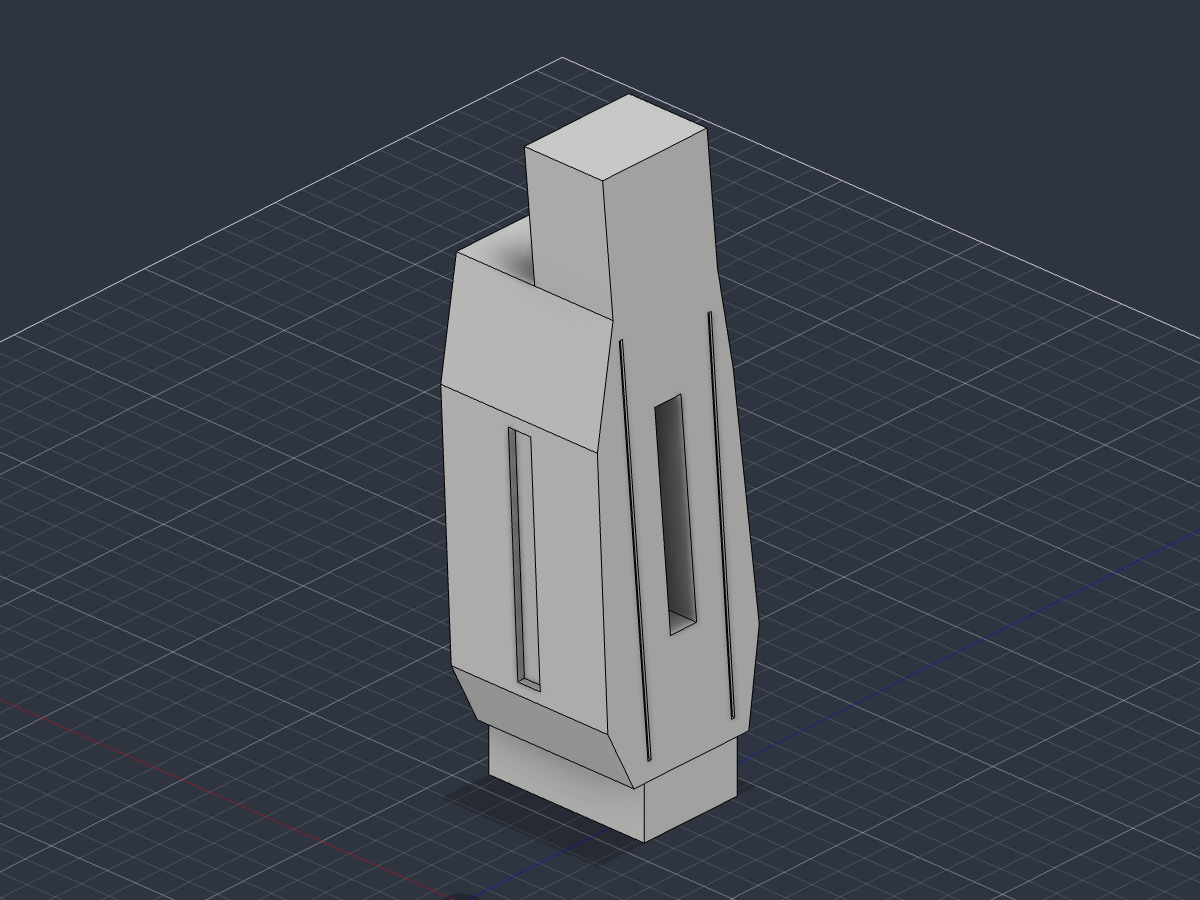
\includegraphics[width = \linewidth]{part-lower-column.png}\caption{04 Lower column}\end{subfigure}\hfill
  \begin{subfigure}{0.32\linewidth}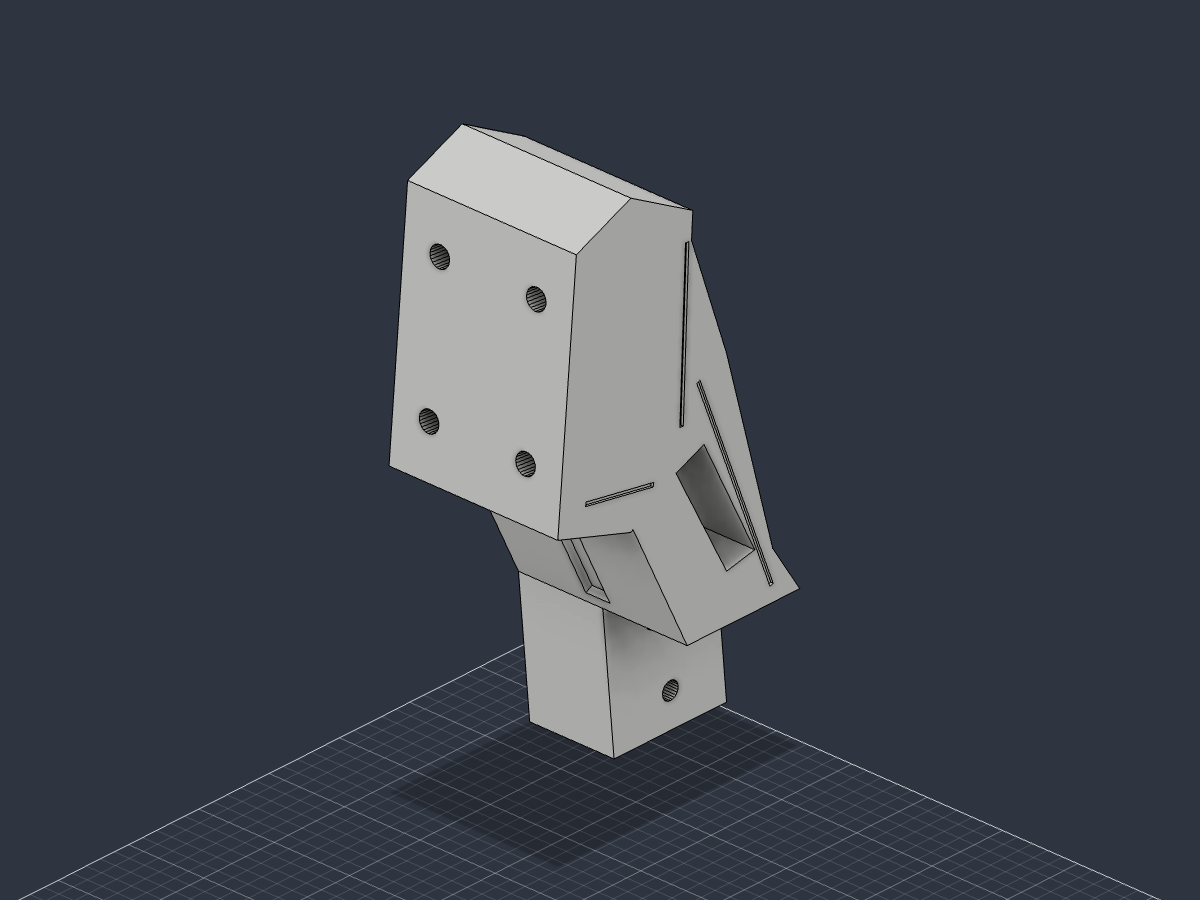
\includegraphics[width = \linewidth]{part-upper-arm.png}\caption{05 Upper arm}\end{subfigure}\hfill
  \begin{subfigure}{0.32\linewidth}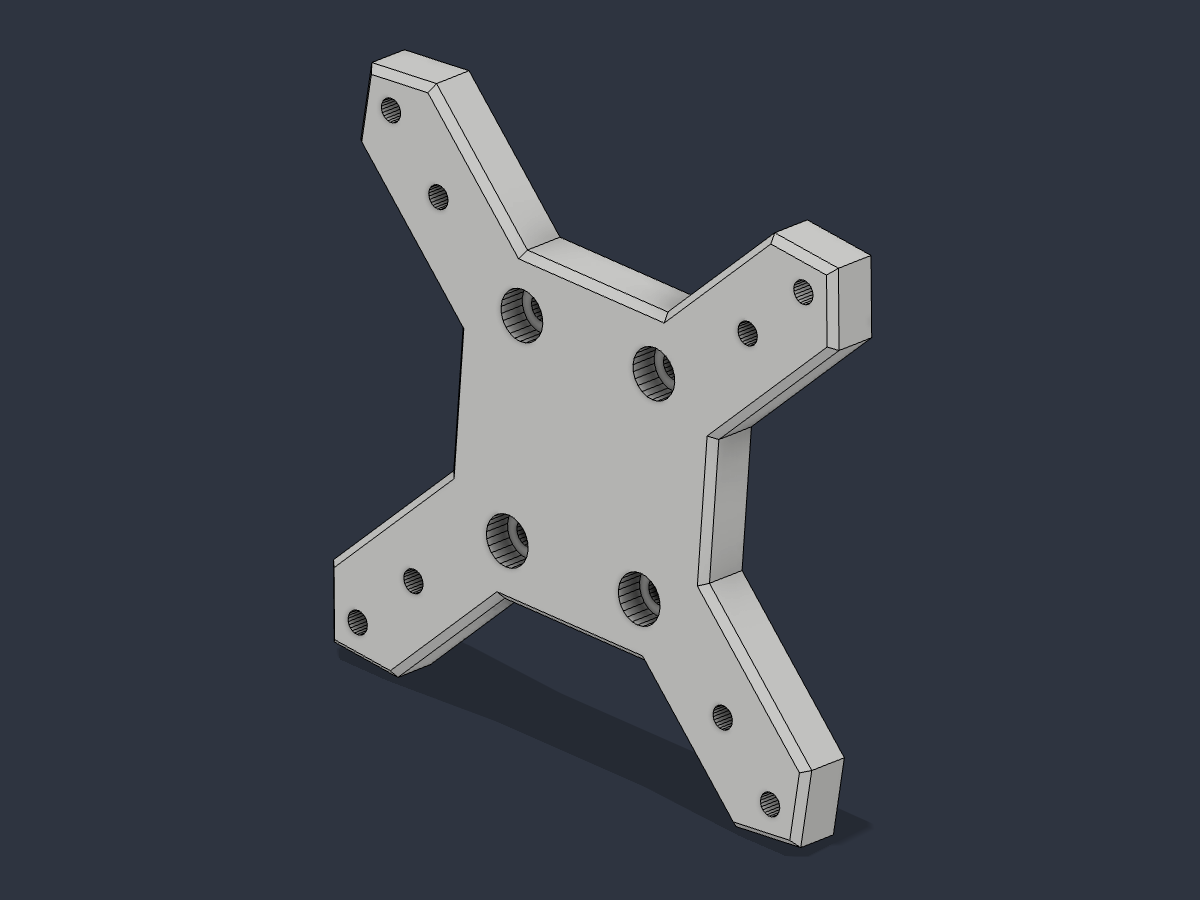
\includegraphics[width = \linewidth]{part-vesa-plate.png}\caption{06 VESA plate}\end{subfigure}
  \caption{Parts, numbered as the STL files in \code{stl/}.}\label{fig:parts}
\end{figure}
